\documentclass[titlepage]{article}
\usepackage{graphicx}
\usepackage[left=1in,right=1in,top=1in,bottom=1in]{geometry}



\author{ Dispoto, Brett\\
	\and
	Kamel, Adham\\
	\and
	Cai, Feiyu\\
}

\title{CS157A Project Proposal}

\begin{document}
	\maketitle
	\section{Project Overview}
	\subsection{Application Overview}
	Our team will be developing a database application where users can find free books and are able to download them via multiple formats and leave reviews on those books for other customers to see. The books that the user can see will be ranging from textbooks to novels. A user will be given the option to create an account, or if they already registered, login to their account. After this, the user will be able to search for a specific book, whether that by the title of the book or its ISBN number. If the user does not know the specific book they want to find, they can search for a specific author, or genre. Searches will include filtering options by the first letter of the book title, the first letter of the author, or by the user's favorites. Users can sort search results alphabetically by sorting by the title alphabetically, the author alphabetically, and by book rating.


	In our application, users will be able to leave reviews on books that they have read, which will be seen by other users and possibly influence their decision on their book. These reviews will contain both a comment section and a star rating system. Users will be able to comment how they either liked or disliked the book and give a star rating from one to five. The average star rating and total number of reviews will be displayed next to the book. Users will also be able to share the book they like with others with a shareable link that they can distribute how they please.
	\subsection{Stakeholders and Importnace}
	The stakeholders of our applications will be students who want to find free textbook alternative to the paid bookstore alternative, as well as casual and dedicated book readers who can find free books online and download them for instant reading. This application is important because it provides a streamline way for bookreaders to gain easy access to the books they want and get them in a timely manner

	\section{System Enviroment}

	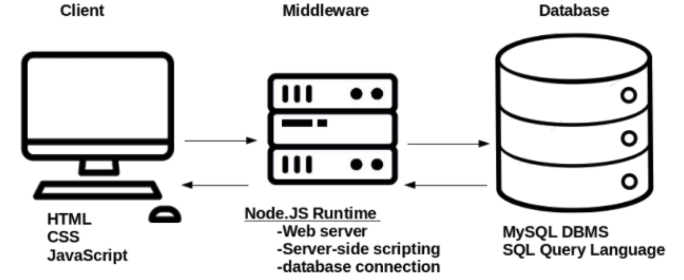
\includegraphics[scale=2.0]{3-tier.png}

	\subsection{Client}
		The presentation layer will be provided via a web browser interface, utilizing languages such as HTML, CSS, and JavaScript. These languages will provide content and interactivity to the database application.
	\subsection{Middleware}
		All middleware will be provided via the Node.js Runtime Environment. This includes:
	\begin{itemize}
		\item A server side scripting language (JavaScript)
		\item Database connection via Node.js MySQL database driver
		\item Node.js build-in web server (HTTP module)
	\end{itemize}

	\subsection{Relational Database}
		The relational database management system (RDBMS) in use will be MySQL, which will be queried via the Structured Query Language (SQL). The following data are examples of what will be stored:
	\begin{itemize}
		\item User information (name, DOB, username, password, site activity, favorites, etc)
		\item Book information (author, ISBN, publisher, date, reviews, etc)
	\end{itemize}

	\subsection{Hardware}
		Although this project will implement a three-tiered database application architecture, all three abstractions will be running on a single local host; this means that the architecture is only virtually three-tiered.

	\section{Functional Requirements}
	The system will provide searching, sorting the shown book lists, reading books, reading reviews, and sharing via email functions from our free textbook database.
	Anonymous visitors can use these functions without signing up for an account. However, signing up for an account with a valid email address will provide more functions.
	A user can sign in his/her account with his/her email address and password. A sign in user will have additional functions such as writing reviews, setting favorite books and having access to their account details page.


\textit{Supported features include:}
	\begin{itemize}
\item	\textbf{Reading:} reading the books itself or its reviews. Input: book information. Output: book content


\item	\textbf{Searching:} searching for book from the provided information. Input: title, author, year of publication, publisher, ISBN, genre, etc. Output: list of books fitting search query.


\item	\textbf{Sorting:} sort the way books are listed. Input: sorting rules such as reviews, alphabetical order, etc.


\item	\textbf{Review:} Give a review and write comments for a book. Input: review and comments. Output: Review and comments are posted on the database that everyone can see


\item	\textbf{Set favorites:} set a book as favorites, the user can see it in his/her profile. Input: “set favorites” button in book details. Output: books stores in the user’s profile.


\item	\textbf{Sharing via email:} sharing book details via email. Input: sharing button in book details. Output: generate share URL link that ready to send via email.

	\end{itemize}



	\section{Non-functional Issues}
	\subsection{Graphical User Interface}
	The GUI of this project will focus on using mouse and keyboard input to trigger the changes of content that will be displayed to user.
	\begin{itemize}
		\item Type of GUI: HTML/JavaScript based
		\item Software to build: Adobe XD
	\end{itemize}
	\subsection{Access Control}
	There are two type of users with different access control:
	\begin{itemize}
		\item Admin: has control of all book contents, can edit, add, and delete books in addition to having typical visitor user access.
		\item Visitor: Only has read access to website content and edit access to their own account.
	\end{itemize}
	\subsection{Security}
	We planned to use MySQL built-in encryption method to encrypt user's information while being stored in a database.




\end{document}
